\documentclass[a4paper,man,biblatex]{apa6}
\usepackage[american]{babel}
\usepackage{csquotes}
\usepackage[backend=biber]{biblatex}
\usepackage[document]{ragged2e}
\setlength{\RaggedRightParindent}{0.5in}
\addbibresource{references.bib}
\usepackage{graphicx}
\usepackage{url}
\usepackage{xpatch}
\xpatchbibdriver{online}
  {\printfield{entrysubtype}}
  {\printfield{entrysubtype}%
   \newunit\newblock
   \printfield{note}}
  {}
  {}

\renewcommand{\abstract}[1]{}

\title{The Rankability of Data}
\shorttitle{The Rankability of Data}
\author{Armant Touche}
\affiliation{Portland State University}
\date{\today}

\begin{document}
\thispagestyle{otherpage}
\setcounter{biburllcpenalty}{7000}
\setcounter{biburlucpenalty}{8000}

%\maketitle

\noindent Name: Armant Touche\newline
\noindent Date: 4/29/2020

\subsection{Description} I wanted to a research article from the Data Science sphere and share with you a common task that affects everyone of us we search the Internet. Imagine how Google, Youtube, or other notable online application present search results to us. A lot of you may have heard of "Youtube's algorithm" but the algorithim is abstract idea that implemented on other online services other than Youtube. Ranking objects or results requires a lot of questioning. Can we trust the Algorithim? Ranking data is used in other applications such as self-driving cars, resource allocation, cybersecurity, and of course, web searches. There are other applications but I wanted to highlight the more common applications. The figure below is an overview of the relationship between rankability and ranking. Rankability is quantifying the

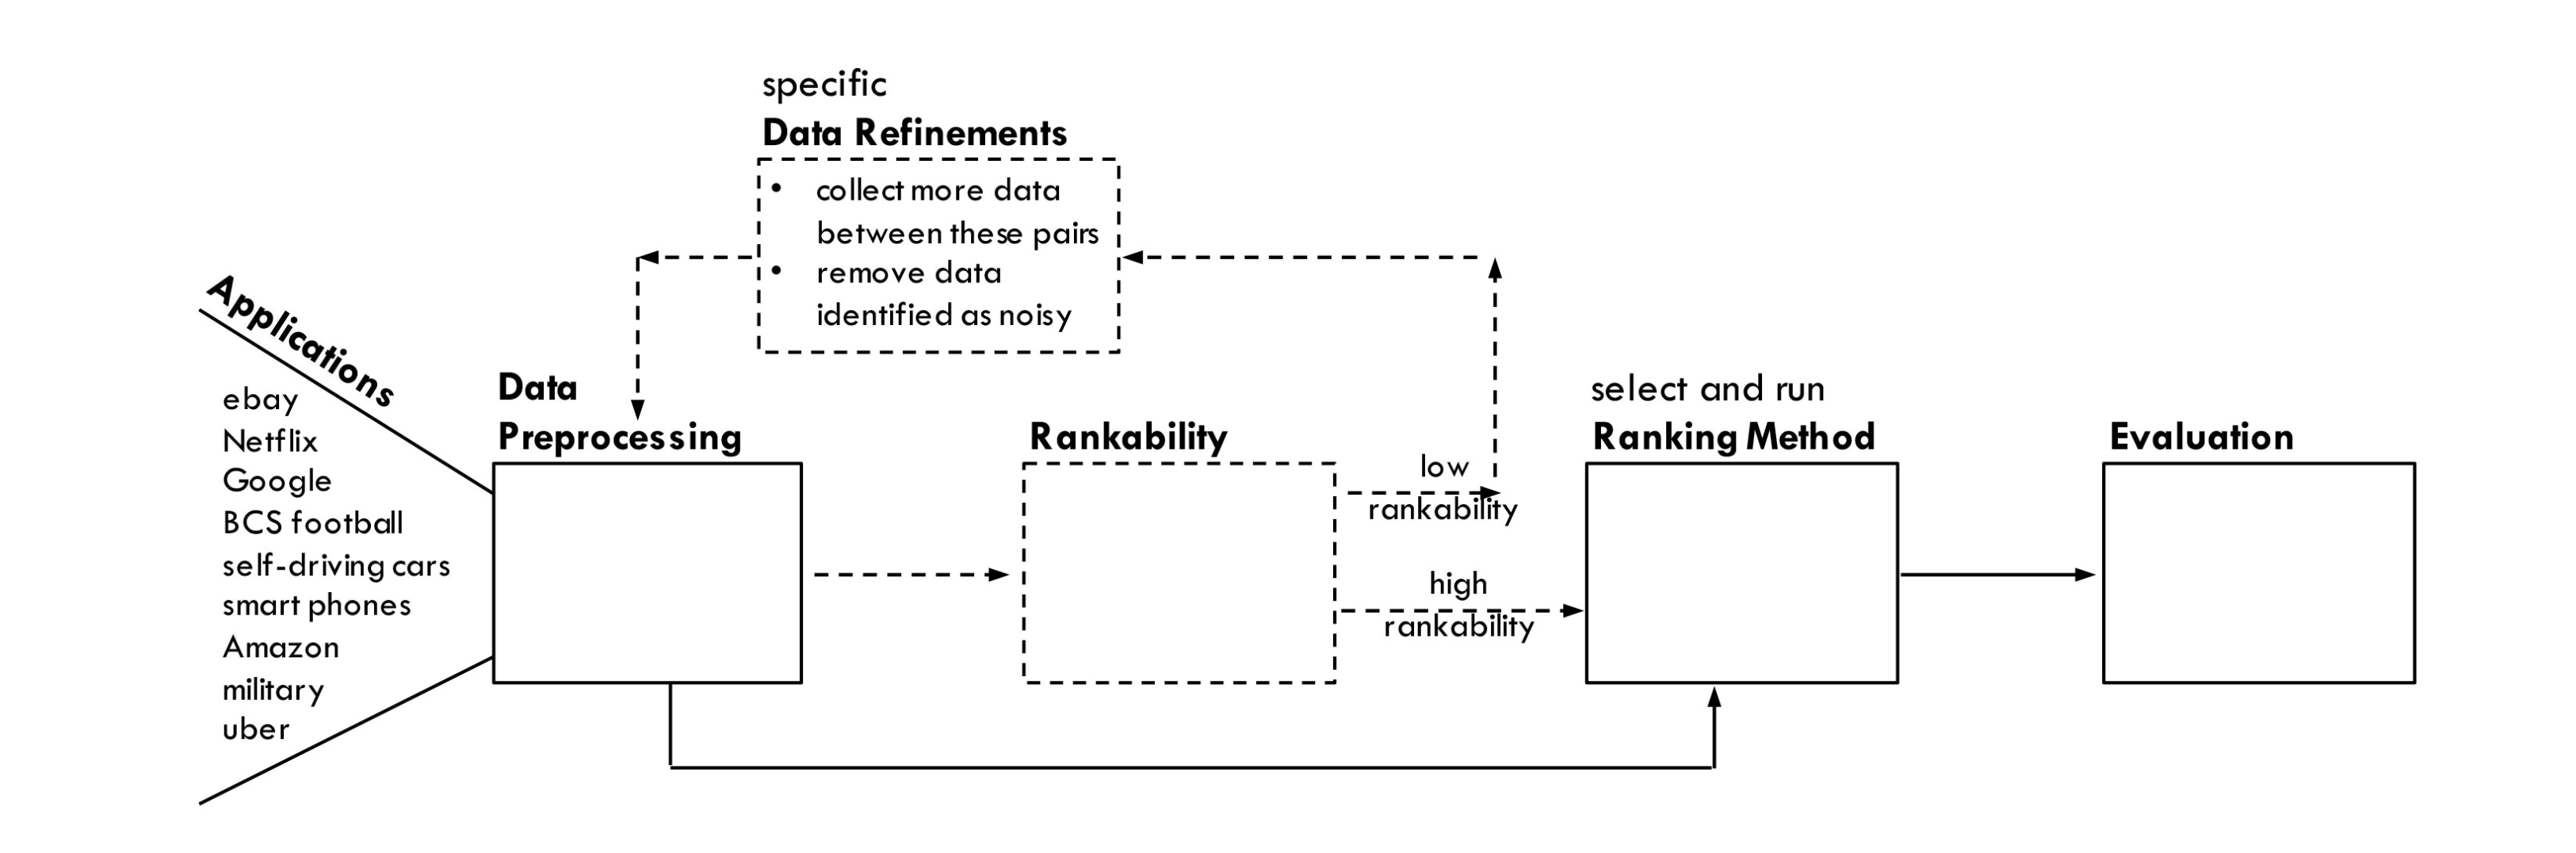
\includegraphics[width=.75\linewidth]{data_pipe}

\subsection{Why} Why this article is important. Overall (400 - 600 words)

\printbibliography

\end{document}
